\documentclass{ieeeaccess}
%
% IEEE Access manuscript
% Patient-level versus nodule-level data partitioning in pulmonary nodule classification
%
\usepackage{cite}
\usepackage{amsmath,amssymb,amsfonts}
\usepackage{algorithmic}
\usepackage{graphicx}
\usepackage{textcomp}
\usepackage{array}
\usepackage{booktabs}

\usepackage{bm}
\makeatletter
\AtBeginDocument{\DeclareMathVersion{bold}
\SetSymbolFont{operators}{bold}{T1}{times}{b}{n}
\SetSymbolFont{NewLetters}{bold}{T1}{times}{b}{it}
\SetMathAlphabet{\mathrm}{bold}{T1}{times}{b}{n}
\SetMathAlphabet{\mathit}{bold}{T1}{times}{b}{it}
\SetMathAlphabet{\mathbf}{bold}{T1}{times}{b}{n}
\SetMathAlphabet{\mathtt}{bold}{OT1}{pcr}{b}{n}
\SetSymbolFont{symbols}{bold}{OMS}{cmsy}{b}{n}
\renewcommand\boldmath{\@nomath\boldmath\mathversion{bold}}}
\makeatother

\def\BibTeX{{\rm B\kern-.05em{\sc i\kern-.025em b}\kern-.08em
    T\kern-.1667em\lower.7ex\hbox{E}\kern-.125emX}}

\begin{document}

\history{Date of submission 09 June 2026.}
\doi{10.1109/ACCESS.2026.DOI}

\title{Patient-Level Versus Nodule-Level Data Partitioning in Pulmonary Nodule Classification: An Empirical Analysis of Performance Bias Across LNDb and LIDC-IDRI Datasets}

\author{\uppercase{Nycolas Mariotto}\authorrefmark{1},
\uppercase{Jadson Gabriel Ferreira}\authorrefmark{1},
\uppercase{Jo\~ao Rafael Almeida de Andrade}\authorrefmark{1},
\uppercase{Jo\~ao Victor Carneiro Faria}\authorrefmark{1},
AND \uppercase{Allan Felipe Fattori Alves}\authorrefmark{1}}
\address[1]{Institute of Biosciences, S\~ao Paulo State University (UNESP), Botucatu, S\~ao Paulo 18618-689, Brazil}

\tfootnote{This work was supported by the Coordena\c{c}\~ao de Aperfei\c{c}oamento de Pessoal de N\'ivel Superior (CAPES), Brazil.}

\markboth
{Mariotto \headeretal: Patient-Level Versus Nodule-Level Data Partitioning in Pulmonary Nodule Classification}
{Mariotto \headeretal: Patient-Level Versus Nodule-Level Data Partitioning in Pulmonary Nodule Classification}

\corresp{Corresponding author: Allan Felipe Fattori Alves (e-mail: allan.alves@unesp.br).}

\begin{abstract}
Deep learning methods for pulmonary nodule classification on the Lung Image Database Consortium (LIDC-IDRI) routinely report accuracies above 95.0\% and areas under the receiver operating characteristic curve above 99.0\%. Most published studies partition data at the nodule or slice level, allowing observations from the same patient to appear in both the training and test splits. This protocol introduces data leakage, which may inflate performance estimates and mislead claims of clinical generalisation. The aim of this study was to empirically quantify the gap between patient-level and nodule-level partitioning in pulmonary nodule classification. Three experimental scenarios of increasing clinical relevance were evaluated under strict patient-level partitioning (80/10/10, stratified): multiclass nodule type classification on the Lung Nodule Database (LNDb) ($n=294$ computed tomography scans), binary malignancy classification on LIDC-IDRI (1018 scans, 4886 malignant and 10\,031 benign annotations), and an end-to-end pipeline incorporating lung and nodule segmentation. Ten convolutional neural network architectures were evaluated individually and as soft-voting ensembles. The best individual accuracy ranged from 82.6\% in the end-to-end pipeline to 92.3\% in the LNDb scenario. The ensemble accuracies were 94.0\%, 88.1\%, and 79.9\% across the three scenarios. These values fall 6 to 14 percentage points below recent literature reporting 93.0--99.0\% accuracy on LIDC-IDRI under nodule-level or unspecified protocols. Ensembles preserved or increased recall in all scenarios, even when the aggregate accuracy decreased. Patient-level partitioning produces realistic but substantially lower performance estimates than nodule-level protocols dominant in the recent literature. Patient-level evaluation should be the methodological standard in pulmonary nodule classification studies.
\end{abstract}

\begin{keywords}
Deep learning, lung neoplasms, medical image analysis, neural networks, pulmonary nodules, computed tomography, data partitioning, reproducibility
\end{keywords}

\titlepgskip=-21pt

\maketitle

\section{Introduction}
\label{sec:introduction}
\PARstart{L}{ung} cancer is the leading cause of cancer-related mortality worldwide, with approximately 1.82 million deaths in 2022 \cite{bray2024}. Low-dose computed tomography (CT) screening reduces lung cancer mortality in high-risk populations \cite{aberle2011}, with pulmonary nodules being the most frequent radiological manifestation of early stage disease and the primary target of screening examinations \cite{macmahon2017,pedrosa2021}.

Deep learning methods for automated nodule detection and classification have become increasingly popular over the past decade. The Lung Image Database Consortium and Image Database Resource Initiative (LIDC-IDRI) \cite{armato2011} are the de facto benchmarks in this field. A recent survey reported that 40 of the 53 papers on pulmonary nodule malignancy classification published between 2017 and 2022 used LIDC-IDRI \cite{lei2022}. Reported performance has progressed rapidly, with several recent studies claiming accuracy above 95.0\% and area under the receiver operating characteristic curve (AUC) values exceeding 99.0\% \cite{liu2024,dhayalini2026,xu2020,zhang2024}. Such performance, if generalisable to clinical practice, would imply that automated nodule classification is essentially solved.

We argue that this conclusion is not appropriate. A systematic examination of the experimental protocols adopted in this literature reveals a methodological inconsistency that has been insufficiently addressed: the unit of data partitioning. In most published studies, training, validation, and test splits are constructed at the nodule or slice level rather than at the patient level. Under this practice, individual two-dimensional slices extracted from the same three-dimensional nodule are randomly distributed across splits, allowing observations from the same patient to appear simultaneously in training, validation, and test sets. Because adjacent slices of the same nodule are nearly identical, and because patient-specific anatomy, body habitus, and scanner-specific artefacts provide indirect identity cues, this protocol introduces data leakage that is rarely acknowledged. Reported performance estimates may primarily reflect the model's capacity to recognise previously seen anatomical context rather than its ability to generalise to new patients.

The magnitude and clinical relevance of this bias remain largely unquantified for pulmonary nodule classification, although it has been documented in adjacent domains of medical imaging \cite{roberts2021,wen2020}. The LNDb Challenge, one of the few large-scale benchmarks enforcing scan-level partitioning by design, concluded that future evaluation frameworks must focus on scan-level, clinically oriented endpoints \cite{pedrosa2021}. Despite this recommendation, patient-level evaluation remains the exception in published comparative work.

In this study, we conduct an empirical analysis of pulmonary nodule classification performance under strict patient-level partitioning across two public datasets and three experimental scenarios of increasing realism, with comparison to recent literature on the same datasets. The intended clinical role of the evaluated systems is triage support in screening contexts. This work is not a proposal of a new state-of-the-art classifier; rather, it is an empirical contribution to the methodological discussion of how pulmonary nodule classification studies should be evaluated to produce performance estimates that translate to clinical practice.

\section{Related Work}
\label{sec:related}
Data leakage in machine learning for medical imaging has received increasing scrutiny. Roberts et al. \cite{roberts2021} audited machine learning models for COVID-19 detection on chest radiographs and CT, identifying widespread methodological flaws, including improper data partitioning, that produced over-optimistic performance. Wen et al. \cite{wen2020} performed a reproducible evaluation of convolutional neural networks for Alzheimer's disease classification on brain magnetic resonance imaging, demonstrating that data leakage between training and test sets at the subject level inflated reported accuracy substantially. These audits established that the unit of partitioning materially affects reported performance in medical imaging.

In pulmonary nodule classification specifically, the LNDb Challenge \cite{pedrosa2021} is among the few benchmarks that enforce scan-level partitioning by design and explicitly recommend clinically oriented, scan-level evaluation endpoints. Most comparative studies on LIDC-IDRI, however, adopt nodule-level or slice-level cross-validation without separating patients across folds \cite{xu2020,alshabi2019}, or do not specify the partitioning unit \cite{xiao2020,mahbod2023,zhang2024}. The present work is positioned as an empirical quantification of the performance gap that this practice introduces, complementing the qualitative concerns raised in prior audits with direct measurements across two datasets and three experimental scenarios.

\section{Materials and Methods}
\label{sec:methods}

\subsection{Datasets}
Two publicly available CT datasets were used. The Lung Nodule Database (LNDb) \cite{pedrosa2021} comprises 294 chest CT examinations collected at a single site in Porto, Portugal, with radiologist annotations of nodule location, size, and morphology. LIDC-IDRI \cite{armato2011} comprises 1018 CT examinations from 1010 patients, accessed through The Cancer Imaging Archive (TCIA), with heterogeneous acquisition protocols, slice thickness, and reconstruction kernels. Each LIDC-IDRI nodule was annotated independently by up to four radiologists in a two-phase blinded protocol, yielding multiple contours per nodule and supporting consensus mask derivation.

\subsection{Patient-Level Partitioning Protocol}
The partitioning protocol is the central methodological feature of this study. All splits were constructed at the patient level: every CT examination, and consequently every slice and nodule annotation derived from it, was assigned to a single split and could not appear in any other split. The split ratio was 80\% training, 10\% validation, and 10\% test, stratified by class label. The random seed was fixed across all experiments (\texttt{random\_state = 42}) for reproducibility. This protocol prevents three forms of leakage documented in the broader medical imaging literature \cite{roberts2021,wen2020}: anatomical redundancy between adjacent slices of the same nodule; patient-specific anatomical context appearing in patches surrounding the nodule; and scanner-specific imaging signatures that may serve as covert identity cues. Fig.~\ref{fig:partition} illustrates the contrast between patient-level and nodule-level protocols.

\begin{figure}[!t]
\centerline{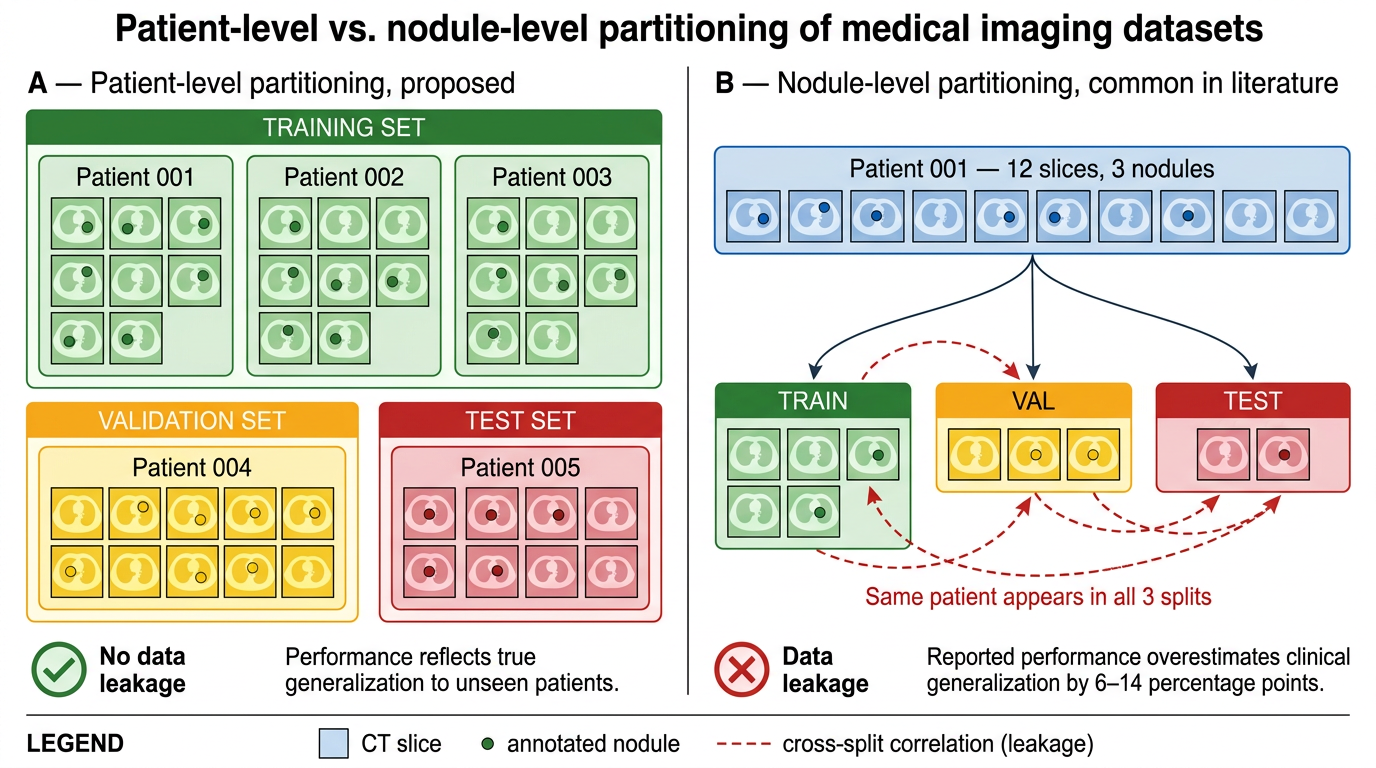
\includegraphics[width=\columnwidth]{fig1.jpg}}
\caption{Schematic comparison of patient-level (proposed) and nodule-level (common in the literature) partitioning protocols. Patient-level partitioning confines all slices and nodules from a given patient to a single split, preventing data leakage. Nodule-level partitioning distributes slices from the same patient across multiple splits, allowing the model to exploit patient-specific anatomical context and scanner-specific artefacts.}
\label{fig:partition}
\end{figure}

For comparability across prior work, the same partitioning logic was applied to all three experimental scenarios. In Experiment 3, due to the absence of an externally separated patient-level test cohort in the available data structure at the time of experimentation, evaluation was performed on the validation split (20\% of the dataset, recreated deterministically with the same \texttt{random\_state}). This constraint is explicitly disclosed as a limitation.

\subsection{Data Curation and Preprocessing}
LIDC-IDRI consensus masks were derived from individual radiologist contours using a 50\% majority voting rule: a voxel was assigned to the final mask if at least two of four annotators marked it as belonging to the nodule \cite{reeves2012}. Binary classification labels were derived from the average radiologist malignancy score per nodule: scores of 4 or 5 were assigned to the malignant class and scores of 1 or 2 to the benign class. Nodules with average score equal to 3 (ambiguous) were excluded. The resulting class distribution comprised 4886 malignant annotations (24.5\%) and 10\,031 benign annotations (50.3\%); 5035 ambiguous annotations (25.2\%) were excluded. The malignant-to-benign ratio in the binary classification dataset was approximately 1:2.05.

CT intensities in Hounsfield Units (HU) were windowed using a lung window (width 1600 HU, level $-600$ HU), clipped to the windowed range, and rescaled to the $[0, 1]$ interval. The final input size was $256 \times 256 \times 3$ pixels. Augmentation was applied during training only and included rotations up to $\pm 30^{\circ}$, translations up to 30\% of the image dimension, shear 0.3, zoom 0.3, and horizontal flipping.

\subsection{Network Architectures and Ensemble}
Networks were selected to span established families: ResNet \cite{he2016}, DenseNet \cite{huang2017}, EfficientNet \cite{tan2019}, Xception \cite{chollet2017}, InceptionResNet \cite{szegedy2017}, ConvNeXt \cite{liu2022}, and VGG \cite{simonyan2015}. Experiment 1 (LNDb multiclass) evaluated 10 architectures: VGG19, InceptionResNetV2, InceptionV3, Xception, ResNet50V2, ResNet101V2, ResNet152V2, DenseNet121, DenseNet169, and DenseNet201. Experiment 2 (LIDC-IDRI binary) evaluated 9 architectures: EfficientNetB7, EfficientNetB4, EfficientNetV2-L, DenseNet121, DenseNet201, ConvNeXtLarge, InceptionResNetV2, ResNet101, and ResNet50. Experiment 3 (end-to-end) evaluated 4: EfficientNetB3, ResNet50, DenseNet121, and InceptionResNetV2. All networks were initialised with ImageNet-pretrained weights. The classification head was reinitialised: two fully connected layers of 128 units with rectified linear unit (ReLU) activation, followed by a final layer with sigmoid (binary) or softmax (multiclass) activation. Fig.~\ref{fig:design} and Fig.~\ref{fig:pipelines} summarise the three experimental scenarios.

\begin{figure*}[!t]
\centerline{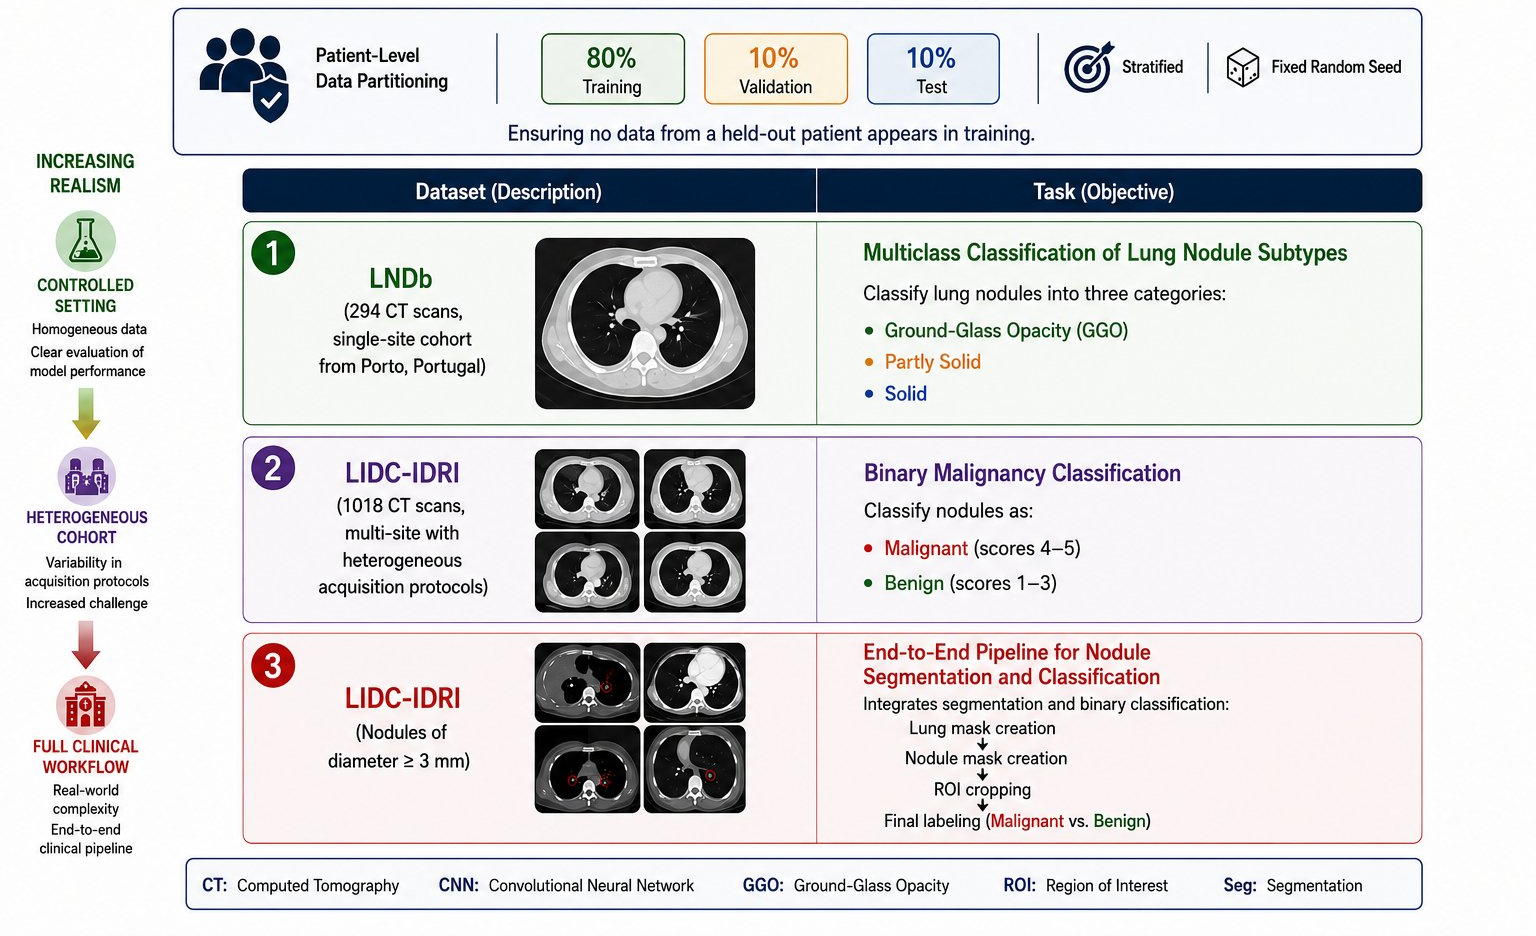
\includegraphics[width=0.92\textwidth]{fig2.png}}
\caption{Experimental design under strict patient-level partitioning: datasets, tasks, and partitioning protocol. Three scenarios of increasing realism are evaluated: multiclass classification on LNDb (single-site cohort), binary malignancy classification on LIDC-IDRI (multi-site cohort), and an end-to-end pipeline on LIDC-IDRI restricted to nodules with diameter $\geq 3$ mm. The same 80/10/10 patient-level split logic applies across all scenarios.}
\label{fig:design}
\end{figure*}

\begin{figure*}[!t]
\centerline{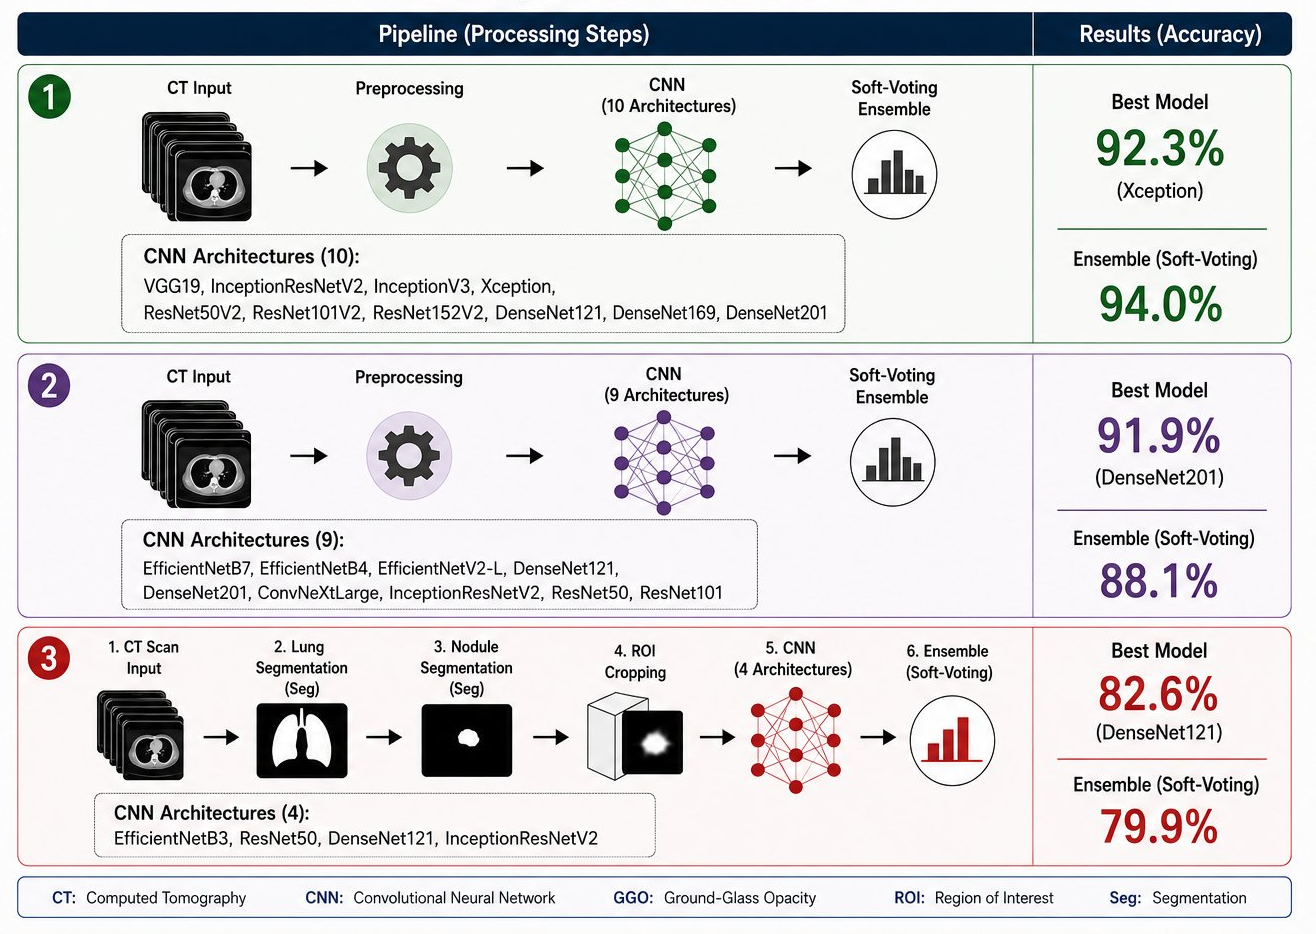
\includegraphics[width=0.92\textwidth]{fig3.png}}
\caption{Processing pipelines and classification results for each experimental scenario. Best individual model and soft-voting ensemble accuracies are reported for each configuration. Convolutional neural network architecture lists detail the models evaluated in each experiment.}
\label{fig:pipelines}
\end{figure*}

Training used the Adam optimiser, initial learning rate $1\times10^{-4}$, batch size 32, binary cross-entropy or categorical cross-entropy loss as appropriate, ReduceLROnPlateau (factor 0.1, patience 5) monitoring validation loss, and early stopping (patience 10), to a maximum of 30 epochs. Soft-voting ensembles were constructed from the top-performing individual models on the validation set, defined as the average of predicted class probabilities, with final class assignment by argmax (multiclass) or a threshold of 0.5 (binary).

\subsection{Evaluation}
Performance was reported using accuracy, precision, recall, and F1-score with macro-averaging across classes. We acknowledge that AUC, bootstrap confidence intervals, and McNemar tests between classifiers are standard expectations in this domain; the intermediate probabilistic predictions from the experimental runs were not preserved at the time of completion of this study, precluding their computation. This limitation is discussed in Section~\ref{sec:limitations}. All results correspond to the held-out test split (Experiments 1 and 2) or held-out validation split (Experiment 3), with no test-set adaptation of hyperparameters at any stage. Implementation used TensorFlow/Keras with scikit-learn for stratified partitioning and pylidc for LIDC-IDRI annotation access.

\section{Results}
\label{sec:results}

\subsection{Multiclass Nodule Type Classification on LNDb}
Individual model accuracy ranged from 79.8\% (DenseNet121) to 92.3\% (Xception). The three top-performing models (Xception, ResNet50V2, and InceptionResNetV2) were selected to compose the ensemble via soft voting. The ensemble achieved 94.0\% accuracy, exceeding the best individual model by 1.7 percentage points. Per-class performance is summarised in Table~\ref{tab:lndb}. Performance on the ground-glass opacity (GGO) class was particularly strong (ensemble precision 97.0\%, recall 91.0\%). The partly-solid class, traditionally the most challenging due to its morphological intermediate nature, achieved an F1-score of 87.0\% in the ensemble configuration.

\begin{table}[!t]
\caption{Per-Class Performance for the Top Three Individual Models and the Soft-Voting Ensemble in the LNDb Multiclass Scenario}
\label{tab:lndb}
\centering
\begin{tabular}{@{}llccc@{}}
\toprule
\textbf{Model} & \textbf{Class} & \textbf{Precision} & \textbf{Recall} & \textbf{F1-score} \\
\midrule
ResNet50V2 & GGO & 97.0\% & 80.0\% & 88.0\% \\
 & Partly solid & 77.0\% & 67.0\% & 72.0\% \\
 & Solid & 81.0\% & 98.0\% & 88.0\% \\
InceptionResNetV2 & GGO & 94.0\% & 84.0\% & 89.0\% \\
 & Partly solid & 80.0\% & 78.0\% & 79.0\% \\
 & Solid & 86.0\% & 93.0\% & 89.0\% \\
Xception & GGO & 96.0\% & 90.0\% & 92.0\% \\
 & Partly solid & 85.0\% & 93.0\% & 89.0\% \\
 & Solid & 96.0\% & 94.0\% & 88.0\% \\
\textbf{Ensemble} & \textbf{GGO} & \textbf{97.0\%} & \textbf{91.0\%} & \textbf{94.0\%} \\
 & \textbf{Partly solid} & \textbf{86.0\%} & \textbf{89.0\%} & \textbf{87.0\%} \\
 & \textbf{Solid} & \textbf{97.0\%} & \textbf{94.0\%} & \textbf{95.0\%} \\
\bottomrule
\end{tabular}
\end{table}

\subsection{Binary Malignancy Classification on LIDC-IDRI}
Individual model accuracy ranged across the nine evaluated architectures, with DenseNet201 achieving 91.9\%. Other strong performers were InceptionResNetV2 (87.8\%) and ConvNeXtLarge (87.7\%). The ensemble achieved 88.1\% accuracy. In this scenario the ensemble did not surpass the best individual model in aggregate accuracy, but per-class metrics indicated that the ensemble preserved recall at a level comparable to or higher than the constituent models.

\subsection{End-to-End Pipeline on LIDC-IDRI}
The third scenario evaluated a complete pipeline incorporating lung segmentation, nodule segmentation, region-of-interest (ROI) extraction, and binary classification. Only nodules with diameter greater than 3 mm were considered \cite{macmahon2017}. Table~\ref{tab:e2e} reports the results.

\begin{table}[!t]
\caption{Performance of Individual Models and the Ensemble in the End-to-End Pipeline on LIDC-IDRI (Validation Split)}
\label{tab:e2e}
\centering
\begin{tabular}{@{}lcccc@{}}
\toprule
\textbf{Model} & \textbf{Accuracy} & \textbf{Precision} & \textbf{Recall} & \textbf{F1-score} \\
\midrule
EfficientNetB3 & 71.6\% & 51.0\% & 72.0\% & 60.0\% \\
ResNet50 & 80.6\% & 51.0\% & 72.0\% & 60.0\% \\
DenseNet121 & 82.6\% & 76.0\% & 76.0\% & 76.0\% \\
InceptionResNetV2 & 82.4\% & 77.0\% & 78.0\% & 77.0\% \\
\textbf{Ensemble} & \textbf{79.9\%} & \textbf{78.0\%} & \textbf{79.0\%} & \textbf{76.0\%} \\
\bottomrule
\end{tabular}
\end{table}

The best individual model was DenseNet121 (82.6\% accuracy). The ensemble achieved 79.9\% accuracy, lower than the two top individual models, with the highest precision (78.0\%) and recall (79.0\%) among all evaluated configurations. The reduction from Experiment 2 (88.1\% ensemble) to Experiment 3 (79.9\%) is interpretable in terms of error propagation across the cascade: segmentation errors propagate into the classification stage.

\subsection{Comparison With the Literature}
Table~\ref{tab:literature} integrates our results with recent studies on LIDC-IDRI. For each cited study, the partitioning protocol was extracted from the Methods section and classified as patient-level (P), nodule-level (N), or unspecified (U).

\begin{table*}[!t]
\caption{Comparative Analysis of Recent Pulmonary Nodule Classification Studies on LIDC-IDRI Stratified by Partitioning Protocol. U, Unspecified; N, Nodule-Level; P, Patient-Level}
\label{tab:literature}
\centering
\begin{tabular}{@{}llcccccc@{}}
\toprule
\textbf{Study (year)} & \textbf{Method} & \textbf{Partition} & \textbf{Acc.} & \textbf{Recall} & \textbf{F1} & \textbf{AUC} \\
\midrule
Saha \& Prakash 2025 \cite{liu2024} & Stacked ensemble + attention & U & 98.1\% & --- & --- & 99.6\% \\
Dhayalini \& Revathi 2026 \cite{dhayalini2026} & Multiscale Swin Transformer & U & 99.4\% & 99.2\% & 99.1\% & --- \\
Xu et al. 2020 \cite{xu2020} & 3D CNN ensemble multi-scale & N & 92.6\% & 85.5\% & 87.9\% & 94.0\% \\
Xiao et al. 2020 \cite{xiao2020} & CNN ensemble + morphology & U & 93.1\% & 81.8\% & 82.8\% & --- \\
Zhang et al. 2024 \cite{zhang2024} & Local-global hybrid network & U & 94.4\% & 94.3\% & --- & 97.3\% \\
Saied et al. 2023 \cite{mahbod2023} & Radiomics + transfer learning & U & 90.4\% & --- & --- & 96.0\% \\
Pedrosa et al. 2021 \cite{pedrosa2021} & LNDb challenge baseline & P & $\sim$94.0\% & --- & --- & --- \\
Al-Shabi et al. 2019 \cite{alshabi2019} & Local-Global Net & N & --- & --- & --- & 95.6\% \\
\textbf{This work --- Exp. 1 (LNDb)} & \textbf{CNN ensemble (soft voting)} & \textbf{P} & \textbf{94.0\%} & \textbf{91.0\%} & \textbf{92.0\%} & \textbf{---} \\
\textbf{This work --- Exp. 2 (LIDC binary)} & \textbf{CNN ensemble (soft voting)} & \textbf{P} & \textbf{88.1\%} & \textbf{79.0\%} & \textbf{76.0\%} & \textbf{---} \\
\textbf{This work --- Exp. 3 (LIDC E2E)} & \textbf{CNN ensemble + segmentation} & \textbf{P} & \textbf{79.9\%} & \textbf{79.0\%} & \textbf{76.0\%} & \textbf{---} \\
\bottomrule
\end{tabular}
\end{table*}

\begin{figure*}[!t]
\centerline{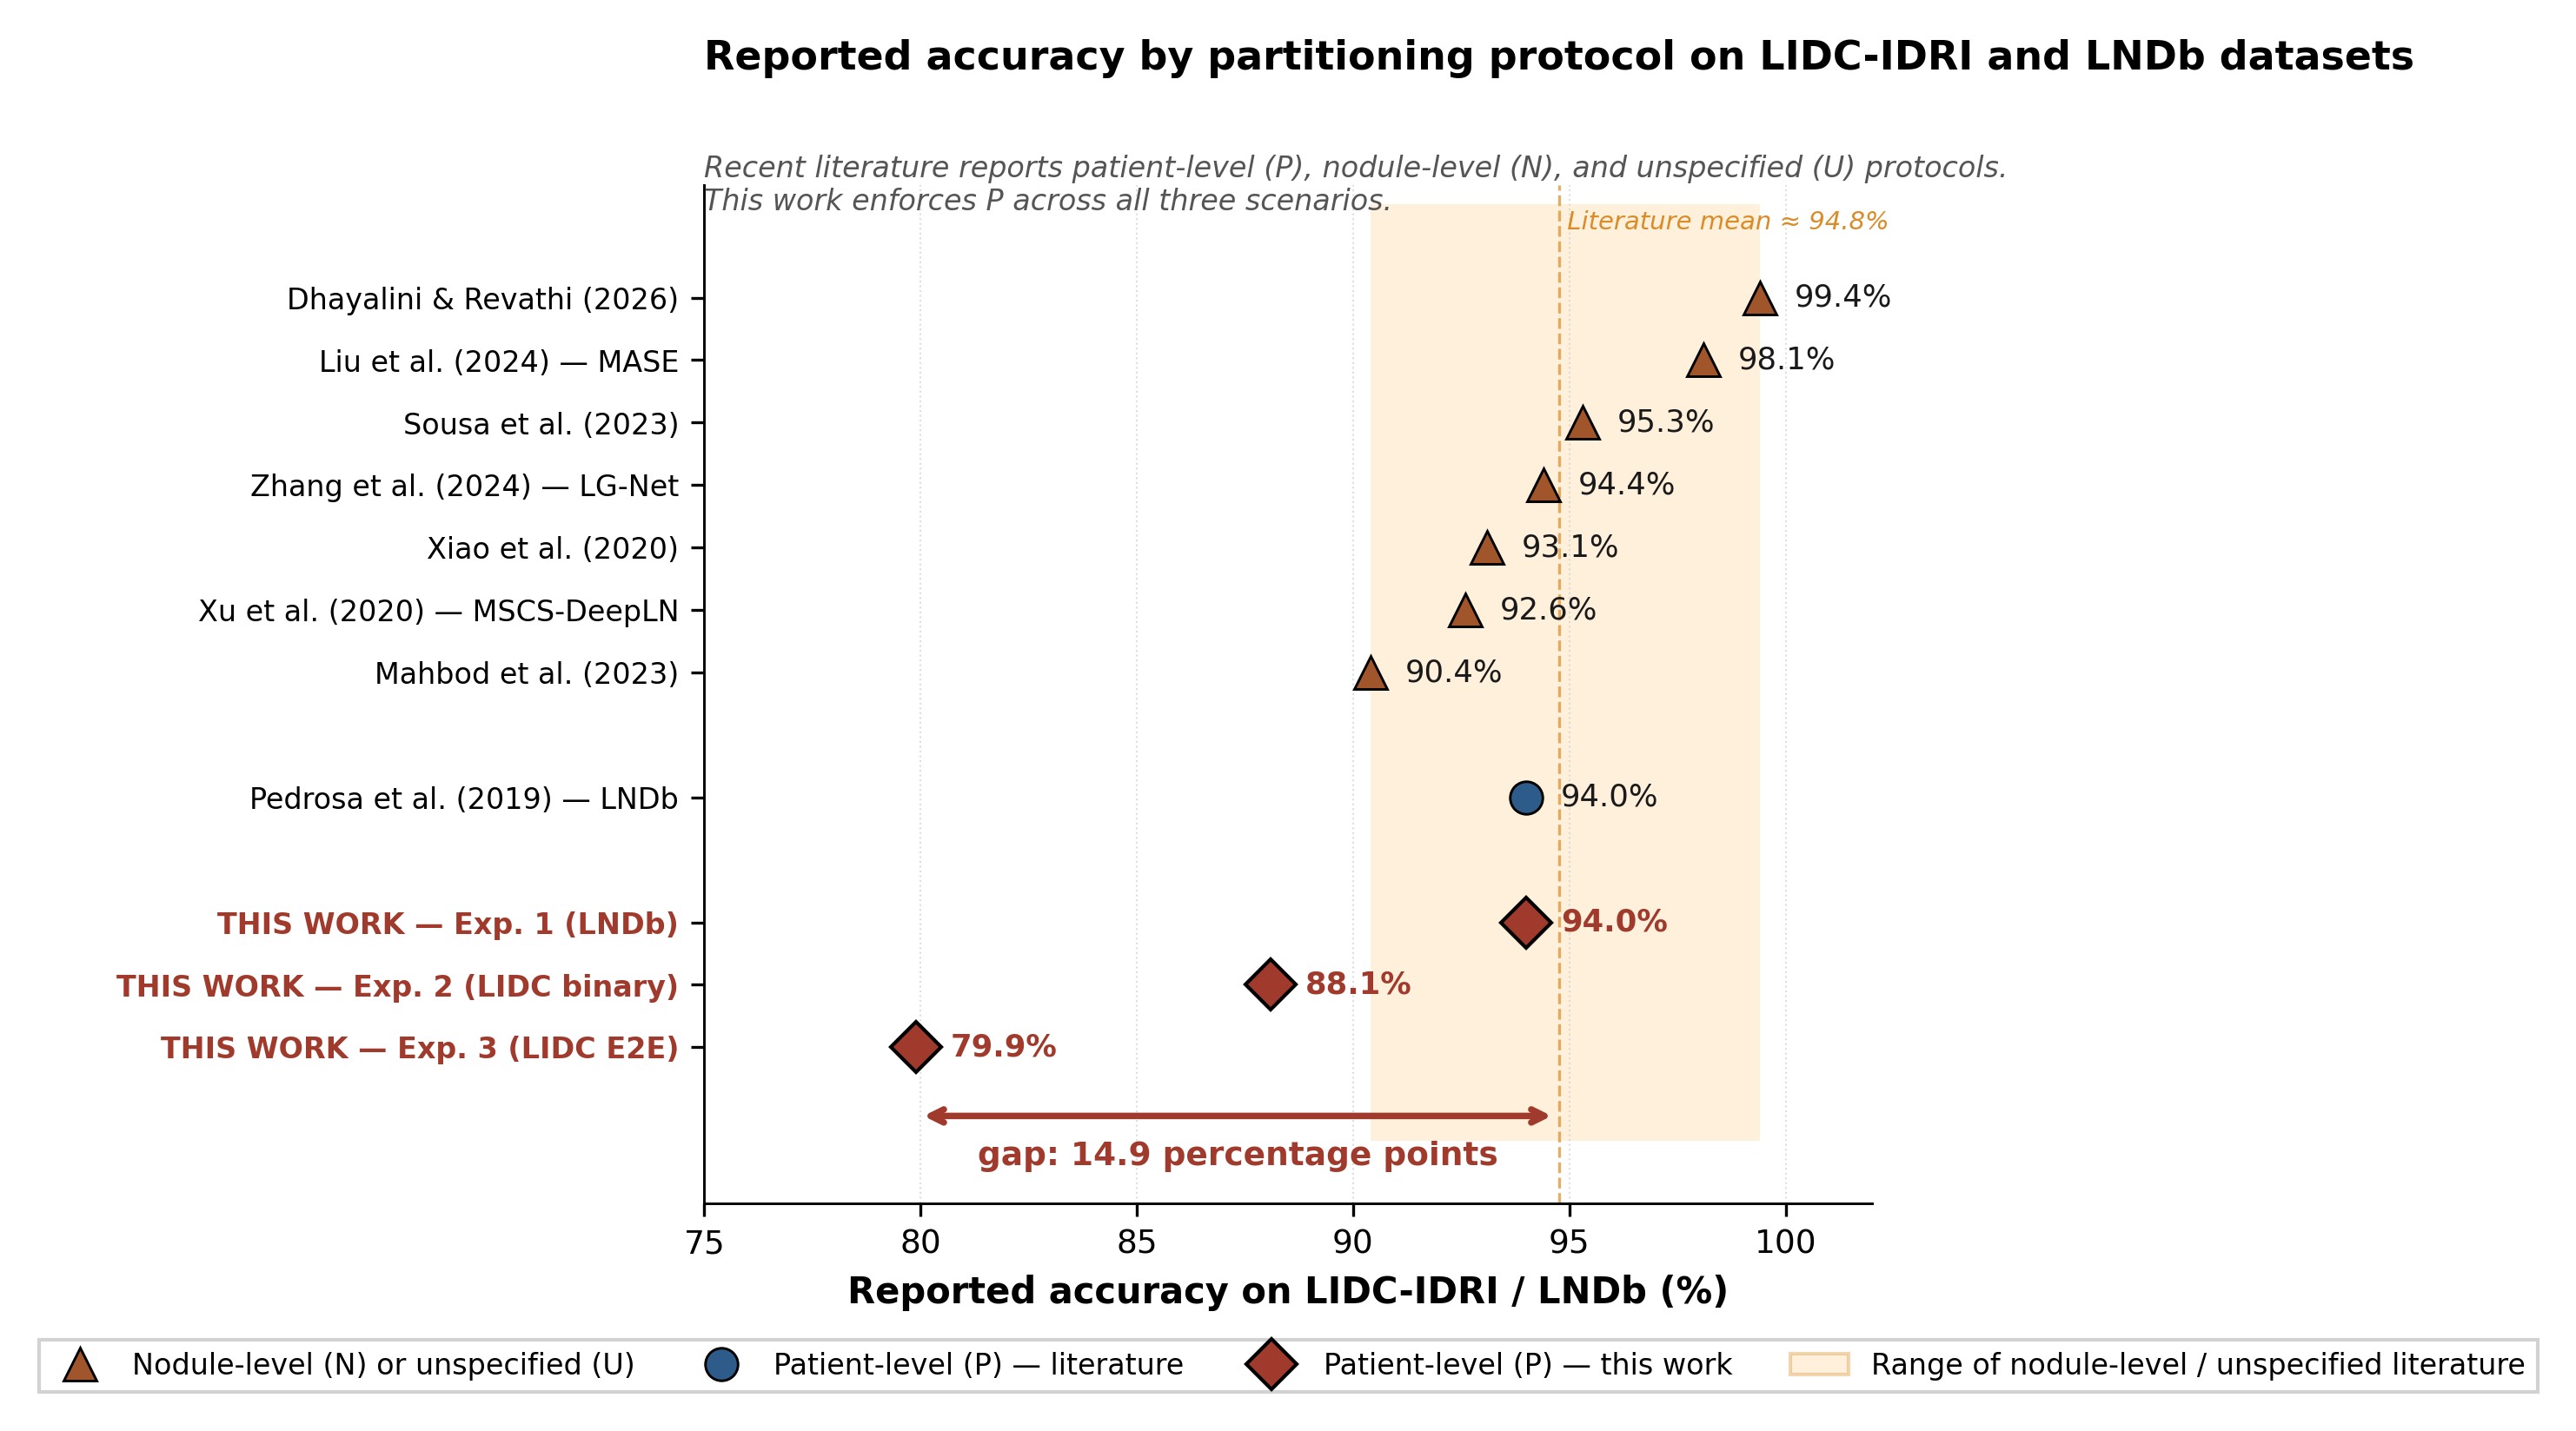
\includegraphics[width=0.85\textwidth]{fig4.png}}
\caption{Reported accuracy by partitioning protocol on the LIDC-IDRI and LNDb datasets. Recent literature studies are stratified by partitioning protocol: nodule-level (N) or unspecified (U), patient-level (P) literature, and the three patient-level scenarios of this study. The orange band indicates the range spanned by the nodule-level and unspecified studies, and the dashed line indicates their mean accuracy. The 14.9 percentage-point gap between the present study's most realistic scenario (Experiment 3) and the literature mean visualises the magnitude of bias introduced by relaxed partitioning protocols.}
\label{fig:forest}
\end{figure*}

Across studies that do not explicitly enforce patient-level partitioning (categories N and U), reported accuracies cluster between 90.0\% and 99.0\%, with a mean of approximately 94.0\% (Fig.~\ref{fig:forest}). The only study in the comparison that explicitly enforces scan-level partitioning, the LNDb Challenge baseline \cite{pedrosa2021}, reports approximately 94.0\% accuracy on LNDb, aligning closely with our Experiment 1 result (94.0\%) on the same dataset. In contrast, our patient-level results on LIDC-IDRI fall in the 79.9--88.1\% range, representing a gap of 6 to 14 percentage points relative to the literature mean of studies using nodule-level or unspecified protocols. The monotonic degradation across our three scenarios (94.0\% $\rightarrow$ 88.1\% $\rightarrow$ 79.9\%) corresponds to increasing realism: controlled single-site multiclass classification, heterogeneous binary classification, and full clinical workflow including segmentation.

\section{Discussion}
\label{sec:discussion}

\subsection{Principal Findings and Consistency of the Partitioning Bias}
The central observation of this study was the systematic gap between the performance estimates obtained under patient-level partitioning and those reported in the recent literature using nodule-level or unspecified protocols. Across our three scenarios, the best individual classifier achieved 92.3\% accuracy in the multiclass LNDb setting, 91.9\% in the binary LIDC-IDRI setting, and 82.6\% in the end-to-end pipeline. The corresponding ensemble accuracies were 94.0\%, 88.1\%, and 79.9\%. As Fig.~\ref{fig:forest} shows, these values fall 6 to 14 percentage points below the literature mean of recent comparable studies on LIDC-IDRI, which reports accuracies between 93.0\% and 99.0\%. The only study in our comparison that explicitly enforces scan-level partitioning, the LNDb Challenge baseline of Pedrosa et al. \cite{pedrosa2021}, reports accuracy in the same range as ours (around 94.0\%), consistent with the hypothesis that the gap is primarily attributable to partitioning rather than to differences in architecture, preprocessing, or class definition.

The gap is reproduced across two independent datasets (LNDb and LIDC-IDRI) and three experimental scenarios, despite differences in dataset size, acquisition protocols, and annotation strategies. It widens monotonically as the experimental scenario becomes more realistic: smallest in the multiclass LNDb experiment, largest in the end-to-end LIDC-IDRI pipeline that incorporates segmentation error and full LIDC-IDRI heterogeneity. The magnitude observed is consistent with data leakage gaps documented in adjacent domains of medical imaging, including chest radiography \cite{roberts2021} and brain magnetic resonance imaging \cite{wen2020}, where systematic methodological audits have produced 5 to 20 point reductions when leakage-free protocols are enforced.

\subsection{Mechanisms of Leakage at the Nodule Level}
Several mechanisms contribute to the inflation of reported performance under nodule-level partitioning. Anatomical redundancy across adjacent slices generates highly correlated training examples that, when randomly assigned to splits, produce near-duplicates in both training and test sets; a model trained under this regime can interpolate between memorised slices rather than learning generalisable features of malignancy. Patient-level anatomical context, including organs, ribs, vasculature, and body habitus, appears as background in patches surrounding the nodule and is unique to each patient; the model can learn to associate background features with labels in a way that is not transferable to unseen patients. Scanner-specific imaging signatures, including noise characteristics, reconstruction kernel artefacts, and slice-thickness patterns, vary systematically across acquisition sites and may serve as covert identity cues. Nodule-level protocols therefore evaluate a hybrid task that combines true generalisation with patient and scanner re-identification.

\subsection{Recall Preservation in Ensembles}
A secondary finding concerns the behaviour of soft-voting ensembles under realistic evaluation. In the LIDC-IDRI binary scenario, the ensemble produced lower aggregate accuracy than the best single model (88.1\% versus 91.9\%) but maintained or increased recall relative to lower-performing constituent models. In the end-to-end pipeline, the ensemble achieved the highest recall (79.0\%) among all configurations while reducing accuracy by approximately 3 percentage points compared with the best single model. Clinically, this trade-off is favourable for triage applications, where missed malignancies (false negatives) carry substantially greater cost than false alarms. Ensemble strategies should be reported using recall and class-specific metrics rather than aggregate accuracy alone.

\subsection{Limitations}
\label{sec:limitations}
Several limitations qualify these findings. AUC and formal pairwise statistical tests between classifiers could not be computed because the intermediate probabilistic predictions from the experimental runs were not preserved at the time of completion of this study. LIDC-IDRI malignancy labels reflect subjective radiologist scoring rather than histopathological confirmation, and the label noise introduced by this protocol has been shown to affect downstream model performance \cite{lei2022}; our binarisation criterion (scores 4--5 as malignant, 1--2 as benign) follows established practice but inherits this limitation. The analysis is restricted to two public datasets of broadly similar origin (North American and European cohorts) and does not address whether the partitioning bias varies systematically across populations or scanner vendors. The end-to-end pipeline of Experiment 3 uses an internal validation split rather than a held-out test cohort at the patient level, due to constraints in the dataset organisation at the time of experimentation. No exhaustive grid search was performed over architectures or training regimes, and the relative ordering of the evaluated architectures should be interpreted as a snapshot rather than a definitive ranking.

\subsection{Recommendations for the Field}
We make three recommendations for future work. First, patient-level partitioning should become the methodological default for pulmonary nodule classification studies; studies that operate at the nodule or slice level should report this choice explicitly and justify its appropriateness for the intended clinical translation. Second, for benchmarking and comparison with legacy literature, studies could report performance under both protocols to enable interpretation of historical claims. Third, reviewers and editors of medical imaging journals could request explicit disclosure of the partitioning unit. These recommendations align with the conclusions of Pedrosa et al. \cite{pedrosa2021} for the LNDb Challenge and with recent methodological audits in medical imaging, although practical adoption remains uneven.

\section{Conclusion}
\label{sec:conclusion}
Performance estimates obtained under strict patient-level partitioning fall 6 to 14 percentage points below the values typically reported in the recent literature on the same datasets, where partitioning is most commonly performed at the nodule or slice level. This gap is reproducible across two independent cohorts and across scenarios of increasing realism and is consistent in magnitude with data leakage gaps documented in adjacent domains of medical imaging. Soft-voting ensembles preserved or increased recall, which is the clinically relevant metric for screening, even when aggregate accuracy decreased. Patient-level partitioning should be the methodological standard for pulmonary nodule classification studies, and benchmark studies should report performance under both protocols to enable interpretation of historical claims in the context of contemporary methodological standards.

\section*{Author Contributions}
N. Mariotto: conceptualization, investigation, methodology, validation, visualization, formal analysis, data curation, writing---original draft, writing---review and editing, and supervision. J. G. Ferreira: investigation, methodology, and data curation. J. R. Almeida de Andrade: data curation, methodology, and investigation. J. V. Carneiro Faria: methodology, data curation, and investigation. A. F. Fattori Alves: project administration, supervision, funding acquisition, formal analysis, data curation, writing, original draft, and writing, review, and editing.

\section*{Acknowledgment}
The authors acknowledge the LIDC-IDRI and LNDb consortia for making their datasets publicly available. During the preparation of this work, the authors used a generative artificial intelligence large language model to assist with manuscript drafting, structural editing, and language refinement, and generative AI design tools to assist with the preparation of schematic figures (Fig.~\ref{fig:design} and Fig.~\ref{fig:pipelines}). All AI-assisted outputs were reviewed, edited, and verified by the authors, who take full responsibility for the content and integrity of this manuscript. All scientific content, experimental data, methodological decisions, results, interpretations, and citations are the authors' own.

\section*{Data Availability}
The LIDC-IDRI dataset is publicly available through The Cancer Imaging Archive (TCIA) at \url{https://www.cancerimagingarchive.net/collection/lidc-idri/}. The LNDb dataset is publicly available at \url{https://zenodo.org/records/6613714}. The patient-level partitioning indices and evaluation code are available from the corresponding author upon reasonable request.

\begin{thebibliography}{00}

\bibitem{bray2024} F. Bray, M. Laversanne, H. Sung \textit{et al.}, ``Global cancer statistics 2022: GLOBOCAN estimates of incidence and mortality worldwide for 36 cancers in 185 countries,'' \textit{CA Cancer J. Clin.}, vol. 74, no. 3, pp. 229--263, 2024.

\bibitem{aberle2011} D. R. Aberle, A. M. Adams, C. D. Berg \textit{et al.}, ``Reduced lung-cancer mortality with low-dose computed tomographic screening,'' \textit{New England J. Med.}, vol. 365, no. 5, pp. 395--409, 2011.

\bibitem{macmahon2017} H. MacMahon, D. P. Naidich, J. M. Goo \textit{et al.}, ``Guidelines for management of incidental pulmonary nodules detected on CT images: from the Fleischner Society 2017,'' \textit{Radiology}, vol. 284, no. 1, pp. 228--243, 2017.

\bibitem{pedrosa2021} J. Pedrosa, G. Aresta, C. Ferreira \textit{et al.}, ``LNDb challenge on automatic lung cancer patient management,'' \textit{Med. Image Anal.}, vol. 70, p. 102027, 2021.

\bibitem{armato2011} S. G. Armato, 3rd, G. McLennan, L. Bidaut \textit{et al.}, ``The Lung Image Database Consortium (LIDC) and Image Database Resource Initiative (IDRI): a completed reference database of lung nodules on CT scans,'' \textit{Med. Phys.}, vol. 38, no. 2, pp. 915--931, 2011.

\bibitem{lei2022} H. Lei, W. Liu, H. Xie, B. Zhao, G. Yue, and B. Lei, ``Re-thinking and re-labeling LIDC-IDRI for robust pulmonary cancer prediction,'' \textit{arXiv:2207.14238}, 2022.

\bibitem{liu2024} U. Saha and S. Prakash, ``Multi-attention stacked ensemble for lung cancer detection in CT scans,'' \textit{arXiv:2507.20221}, 2025.

\bibitem{dhayalini2026} M. Dhayalini and B. Revathi alias Ponmozhi, ``Multi-phase deep learning framework with multiscale adaptive Swin transformer and embedding attention for precision lung nodule detection and classification,'' \textit{Sci. Rep.}, vol. 16, p. 1652, 2026, doi: 10.1038/s41598-025-31147-2.

\bibitem{xu2020} X. Xu, C. Wang, J. Guo \textit{et al.}, ``MSCS-DeepLN: evaluating lung nodule malignancy using multi-scale cost-sensitive neural networks,'' \textit{Med. Image Anal.}, vol. 65, p. 101772, 2020.

\bibitem{zhang2024} X. Zhang, P. Yang, J. Tian, F. Wen, X. Chen, and T. Muhammad, ``Classification of benign and malignant pulmonary nodule based on local-global hybrid network,'' \textit{J. Xray Sci. Technol.}, vol. 32, no. 1, pp. 1--15, 2024.

\bibitem{roberts2021} M. Roberts, D. Driggs, M. Thorpe \textit{et al.}, ``Common pitfalls and recommendations for using machine learning to detect and prognosticate for COVID-19 using chest radiographs and CT scans,'' \textit{Nature Mach. Intell.}, vol. 3, no. 3, pp. 199--217, 2021.

\bibitem{wen2020} J. Wen, E. Thibeau-Sutre, M. Diaz-Melo \textit{et al.}, ``Convolutional neural networks for classification of Alzheimer's disease: overview and reproducible evaluation,'' \textit{Med. Image Anal.}, vol. 63, p. 101694, 2020.

\bibitem{reeves2012} M. C. Hancock and J. F. Magnan, ``Lung nodule malignancy classification using only radiologist-quantified image features as inputs to statistical learning algorithms: probing the Lung Image Database Consortium dataset with two statistical learning methods,'' \textit{J. Med. Imag.}, vol. 3, no. 4, p. 044504, Dec. 2016, doi: 10.1117/1.JMI.3.4.044504.

\bibitem{he2016} K. He, X. Zhang, S. Ren, and J. Sun, ``Deep residual learning for image recognition,'' in \textit{Proc. IEEE Conf. Comput. Vis. Pattern Recognit. (CVPR)}, 2016, pp. 770--778.

\bibitem{huang2017} G. Huang, Z. Liu, L. van der Maaten, and K. Q. Weinberger, ``Densely connected convolutional networks,'' in \textit{Proc. IEEE Conf. Comput. Vis. Pattern Recognit. (CVPR)}, 2017, pp. 4700--4708.

\bibitem{tan2019} M. Tan and Q. V. Le, ``EfficientNet: rethinking model scaling for convolutional neural networks,'' in \textit{Proc. Int. Conf. Mach. Learn. (ICML)}, 2019, \textit{arXiv:1905.11946}.

\bibitem{chollet2017} F. Chollet, ``Xception: deep learning with depthwise separable convolutions,'' in \textit{Proc. IEEE Conf. Comput. Vis. Pattern Recognit. (CVPR)}, 2017, pp. 1251--1258.

\bibitem{szegedy2017} C. Szegedy, S. Ioffe, V. Vanhoucke, and A. Alemi, ``Inception-v4, Inception-ResNet and the impact of residual connections on learning,'' in \textit{Proc. AAAI Conf. Artif. Intell.}, 2017, \textit{arXiv:1602.07261}.

\bibitem{liu2022} Z. Liu, H. Mao, C. Y. Wu, C. Feichtenhofer, T. Darrell, and S. Xie, ``A ConvNet for the 2020s,'' in \textit{Proc. IEEE Conf. Comput. Vis. Pattern Recognit. (CVPR)}, 2022, pp. 11976--11986.

\bibitem{simonyan2015} K. Simonyan and A. Zisserman, ``Very deep convolutional networks for large-scale image recognition,'' in \textit{Proc. Int. Conf. Learn. Represent. (ICLR)}, 2015, \textit{arXiv:1409.1556}.

\bibitem{xiao2020} N. Xiao, Y. Qiang, M. Bilal Zia, S. Wang, and J. Lian, ``Ensemble classification for predicting the malignancy level of pulmonary nodules on chest computed tomography images,'' \textit{Oncol. Lett.}, vol. 20, no. 1, pp. 401--408, 2020.

\bibitem{mahbod2023} M. Saied, M. Raafat, S. Yehia, and M. M. Khalil, ``Efficient pulmonary nodules classification using radiomics and different artificial intelligence strategies,'' \textit{Insights Imaging}, vol. 14, p. 91, 2023, doi: 10.1186/s13244-023-01441-6.

\bibitem{alshabi2019} M. Al-Shabi, B. L. Lan, W. Y. Chan, K. H. Ng, and M. Tan, ``Lung nodule classification using deep local-global networks,'' \textit{Int. J. Comput. Assist. Radiol. Surg.}, vol. 14, no. 10, pp. 1815--1819, 2019.

\end{thebibliography}

\begin{IEEEbiographynophoto}{Nycolas Mariotto}
received the B.Sc. degree in medical physics and the M.Sc. degree in biomolecular and pharmacological sciences from S\~ao Paulo State University (UNESP), Botucatu, Brazil, where he is currently pursuing the Ph.D. degree in biomolecular and pharmacological sciences. His research focuses on convolutional neural networks and deep learning applied to medical image analysis, including detection, segmentation, and classification tasks, with an emphasis on methodological rigour and reproducibility.
\end{IEEEbiographynophoto}

\begin{IEEEbiographynophoto}{Jadson Gabriel Ferreira}
is an undergraduate researcher with the Institute of Biosciences, S\~ao Paulo State University (UNESP), Botucatu, Brazil. His research interests include medical image analysis and the application of deep learning to computed tomography data.
\end{IEEEbiographynophoto}

\begin{IEEEbiographynophoto}{Jo\~ao Rafael Almeida de Andrade}
is an undergraduate researcher with the Institute of Biosciences, S\~ao Paulo State University (UNESP), Botucatu, Brazil. His research interests include data curation and methodological aspects of deep learning applied to medical imaging.
\end{IEEEbiographynophoto}

\begin{IEEEbiographynophoto}{Jo\~ao Victor Carneiro Faria}
is an undergraduate researcher with the Institute of Biosciences, S\~ao Paulo State University (UNESP), Botucatu, Brazil. His research interests include the methodology and curation of medical imaging datasets for deep learning.
\end{IEEEbiographynophoto}

\begin{IEEEbiographynophoto}{Allan Felipe Fattori Alves}
received the Ph.D. degree in medical physics and is currently a Professor with the Institute of Biosciences, S\~ao Paulo State University (UNESP), Botucatu, Brazil. His research interests include medical image analysis, computer-aided diagnosis, and the application of machine learning methods to radiological imaging.
\end{IEEEbiographynophoto}

\EOD

\end{document}